\section{Кнезеровские графы}

\mysubsection{Определение. Гипотеза Кнезера}

	Ранее мы уже говорили о графах как об объектах, которые получаются с помощью построения дискретной структуры над некоторым множеством. Так, например, любой граф $G$ является графом пересечений, то есть существует такое множество $S$ и такой набор его подмножеств $\lbrace S_i \rbrace_{i=1}^{n}$, что можно построить биекцию между $V(G)$ и этим набором так, что ребрами соединены вершины тогда и только тогда, когда соответствующие им подмножества $S_i, S_j$ пересекаются.
	
	
\begin{paracol}{2}
	Сейчас мы подойдем с похожей стороны к вопросу задания графов: а именно, скажем, что у нас есть множество $\lbrace 1, 2, 3, \dots, n\rbrace$ и вершинами графа будут все $k$-элементные подмножества этого множества, а соединены будут те два подмножества $A, B$, которые не пересекаются, то есть $A \cap B = \varnothing$. Будем говорить, что это \emph{кнезеровский граф} и обозначать его $KG(n, k)$.
	
	Справа вы можете видеть граф Петерсена, который по совместительству тоже является кнезеровским графом.

\switchcolumn

\begin{center}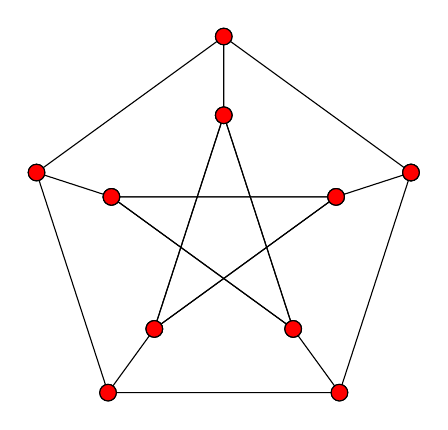
\begin{tikzpicture}
	\tikzstyle{every node}=[circle, draw, fill=red, inner sep=0pt, minimum width=6pt]
	\foreach \x in {18,90,...,306}
    {
    	\draw
    	(\x:1.5) node {} -- (\x+144:1.5)
    	(\x:1.5) node {} -- (\x+216:1.5);
    };
    \foreach \x in {18,90,...,306}
    {
    	\draw
    	(\x:2.5) node {} -- (\x:1.5)
    	(\x:2.5) node {} -- (\x+72:2.5);
    };
    \draw \foreach \x in {18,90,...,306}
    {
    	(\x:1.5) node {}
    };
    \draw (18: 2.5) node {};
\end{tikzpicture}\end{center}
\begin{center}
	\small Рис. \images. Граф $KG(5, 2)$
\end{center}
\end{paracol}
\refstepcounter{images}

	Сразу отметим, что кнезеровские графы обладают не очень привлекательным видом если не выполнено неравенство $k \leqslant \frac{n}{2}$: в противном случае любые два подмножества пересекаются и, следовательно, не будут соединены ребром в графе. Можно уточнить, что 
	$$\forall \; k > \frac{n}{2} \mapsto KG(n, k) \cong O_{{n}\choose{k}}.$$
	
	Теперь вспомним о хроматическом числе графа, то есть о минимальном числе красок, для того чтобы осуществить на графе правильную раскраску. Оказывается, что достаточно просто сформулировать верхнюю оценку на него.
	
\begin{statement}
	Хроматическое число $\chi(G)$ для кнезеровского графа $KG(n, k)$ удовлетворяет следующей оценке 
	$$\chi (KG(n, k)) \leqslant n - 2k + 2.$$
	
	\begin{proof}
	Чтобы доказать неравенство построим явно независимые множества, которые не будут пересекаться, но при этом будут содержать все $k$-элементные подмножества $n$-элементного множества $\lbrace 1, 2, 3, \dots, n\rbrace$. 
	
	Обозначим через $V_1$ "--- те подмножества, которые содержат $1$. Далее из всех подмножеств выберем те, которые содержат $2$, и их объединение обозначим $V_2$... Такими действиями мы получим набор $V_1, V_2, V_3, V_{n - 2k + 1}$, а что дальше? Заметим, что после последней итерации у нас оставшиеся множества получается выборкой $k$ элементов из $(2k - 1)$-элементного множества. Очевидно, что они все пересекаются, так что все вместе образуют последнее $V_{n - 2k + 2}$ независимое множество.
	\end{proof}
\end{statement}

	На самом деле это уникальный случай, когда верхняя оценка на хроматическое число так просто доказывается. Но на этом сказка не заканчивается, хочется ведь знать нижнюю оценку тоже... В $1955$ году Мартин Кнезер тоже задался этим вопросом и сформулировал следующую гипотезу.
	
\begin{hypothesis}[Кнезера]
	Хроматическое число для $KG(n, k)$ в точности равно $n - 2k + 2$.
\end{hypothesis}

	В $1977$ году, благодаря Ласло Ловасу, эта гипотеза стала теоремой, то есть переместилась в список <<доказанных>>.

	Эту оценку можно проверить на примере простых графов.
	
\begin{itemize}
	\item Граф $KG(n, 1) \cong K_n$, поэтому его хроматическое число равно $n$. Оценка же дает как раз это числ: $n - 2 \cdot 1 + 2 = n$. 
	\item Граф $KG(2n, n)$ есть ни что иное, как объединение $K_2$, то есть его хроматическое число равно двум, что равно $2n - 2 \cdot n + 2$.
\end{itemize}
	
	Теперь вспомним неравенство, соединяющее в себе хроматическое число и кликовое число:
	$$\chi(G) \geqslant \omega(G).$$
	
	В границах кнезеровских графов достаточно просто найти кликовое число $\omega(G) = \left[ \frac{n}{k}\right]$. В таком случае мы можем выписать следующую нижнюю оценку
	$$\chi(G) \geqslant \omega(G) = \left[ \frac{n}{k} \right].$$
	Она ни в коем случае не претендует на столь же красочный вид, как и гипотеза Кнезера, но при этом она может нам рассказать некоторые интересные факты о кнезеровских графах: например, если $k = \frac{n}{3} + 1$, то в графе нет треугольников, но при этом хроматическое число имеет асимптотику $\Theta(n)$. 




	